% **************************************************************************************************
% ** SPSC Report and Thesis Template
% **************************************************************************************************
%
% ***** Authors *****
% Daniel Arnitz, Paul Meissner, Stefan Petrik
% Signal Processing and Speech Communication Laboratory (SPSC)
% Graz University of Technology (TU Graz), Austria
%
% ***** Changelog *****
% 0.1   2010-01-25   extracted from report template by Daniel Arnitz (not ready yet)
% 0.2   2010-02-08   added thesis titlepage and modified layout (not ready yet)
% 0.3   2010-02-18   added TUG logo and statutory declaration
% 0.4   2010-02-18   moved the information fields below \input{./base/packages} (encoding...)
% 0.5   2010-03-02   added \ShortTitle to fix problems with long thesis titles
%                    added \ThesisType (makes the template suitable for MSc, BSc, PhD, ... Thesis)
% 0.6   2010-06-05   added pagestyle and pagenumbering after frontmatter, packages has now type
% 0.7   2010-09      \Advisors -> \Assessors, inserted frontmatter for thesis
% 0.8   2010-11      added examples
% 0.9   2011-04      \Twosided now {true,false}, scrbook for thesis (\front-, \main-, \backmatter)
%                    added \SpecialNote for titlepage (funding, etc.), added type "homework"
% 0.10  2011-10-18   fixed two typos in \bibliographystyle{} (bug reported by Michael Tauch)
% 0.11  2011-11-09   fixed/modified preamble (bug reported by Michael Tauch)
% 0.12  2012-07-20   added ./base/opt_macros to deal with optional macros
% 0.13  2012-07-27   added \PaperSize
%
% ***** Todo *****
% - Introduction/Usage
% - explain/show preamble (with \thispagestyle, etc)
% - why doesn't \pagestyle work in preamble while \thispagestyle does? (reported by Markus Fr�hle)
% **************************************************************************************************

% **************************************************************************************************
% basic setup

\newcommand{\DocumentType}{homework} % "thesis" / "report" / "homework"
\newcommand{\DocumentLanguage}{en} % "en" / "de"
\newcommand{\PaperSize}{a4paper} % "a4paper" / "letterpaper"
\newcommand{\Twosided}{false} % "true" / "false"

% **************************************************************************************************
% template setup -- do not change these unless you know what you are doing!
\input{./base/packages_\DocumentType}
\input{./base/layout_\DocumentType}
% **************************************************************************************************
% ** SPSC Report and Thesis Template
% **************************************************************************************************
%
% ***** Authors *****
% Daniel Arnitz, Paul Meissner, Stefan Petrik
% Signal Processing and Speech Communication Laboratory (SPSC)
% Graz University of Technology (TU Graz), Austria
%
% ***** Changelog *****
% 0.1   2010-08-09   added \remc and \remq commands, \nxtpar now uses \med- instead of \bigskip
%                    replaced \lastfootnotemark by \oldfootnotemark (generalization),
%                    added \chapternote, set \openingquote to 0.4\textwidth, modified \MAttention,
%                    \xspace for marginpar commands, modified \MDanger and \MQuestion
% 0.2   2010-10-03   added \exp, colors "bk*"
% 0.3   2010-11-16   added \twofigs and \twofigsf
% 0.4   2010-12      added \F (Fourier), \ceil and \floor
% 0.5   2011-01      added chapter/section/figure/table/part reference commands, textrel
% 0.6   2011-03      added \avg, modified bkred, bkgreen, and bkblue colors,
%                    added \medskip to \chapternote, added natural/real/complex/... numbers
%                    added \rapp for references to the appendix
% 0.7   2011-04      removed labels from \new*NoTOC
% 0.8   2012-06      correction of minor typo
%
% ***** Todo *****
% ? prettyref instead of reference commands
%
% **************************************************************************************************



% **************************************************************************************************
% * SECTIONING AND TEXT
% **************************************************************************************************

% new chapter, section, ... plus a few addons
%   part
\newcommand{\newpart}[2]{\FloatBarrier\cleardoublepage\part{#1}\label{part:#2}}%
%   chapter
\newcommand{\newchapter}[2]{\FloatBarrier\chapter{#1}\label{chp:#2}}
\newcommand{\newchapterNoTOC}[1]{\FloatBarrier\stepcounter{chapter}\chapter*{#1}}%
%   section
\newcommand{\newsection}[2]{\FloatBarrier\vspace{5mm}\section{#1}\label{sec:#2}}%
\newcommand{\newsectionNoTOC}[1]{\FloatBarrier\vspace{5mm}\stepcounter{section}\section*{#1}}%
%   subsection
\newcommand{\newsubsection}[2]{\FloatBarrier\vspace{3mm}\subsection{#1}\label{sec:#2}}%
\newcommand{\newsubsectionNoTOC}[1]{\FloatBarrier\vspace{3mm}\stepcounter{subsection}\subsection*{#1}}%
%   subsubsection
\newcommand{\newsubsubsection}[2]{\vspace{2mm}\subsubsection{#1}\label{sec:#2}}%
\newcommand{\newsubsubsectionNoTOC}[1]{\vspace{2mm}\stepcounter{subsubsection}\subsubsection*{#1}}%

% references
%   chapter(s), section(s), appendix
\newcommand{\rchp}[1]{Chapter~\ref{chp:#1}}
\newcommand{\rchps}[1]{Chapters~\ref{chp:#1}}
\newcommand{\rsec}[1]{Section~\ref{sec:#1}}
\newcommand{\rsecs}[1]{Sections~\ref{sec:#1}}
\newcommand{\rappendix}[1]{Appendix~\ref{#1}}
%   figure(s), table(s), listing(s), equation(s)
\newcommand{\rfig}[1]{Fig.~\ref{fig:#1}}
\newcommand{\rfigs}[1]{Figs.~\ref{fig:#1}}
\newcommand{\rtab}[1]{Tab.~\ref{tab:#1}}
\newcommand{\rtabs}[1]{Tabs.~\ref{tab:#1}}
\newcommand{\rlst}[1]{Listing~\ref{lst:#1}}
\newcommand{\rlsts}[1]{Listings.~\ref{lst:#1}}
\newcommand{\req}[1]{(\ref{eq:#1})}

% varioref references
%   chapter(s), section(s)
\newcommand{\vrchp}[1]{Chapter~\vref{chp:#1}}
\newcommand{\vrchps}[1]{Chapters~\vref{chp:#1}}
\newcommand{\vrsec}[1]{Section~\vref{sec:#1}}
\newcommand{\vrsecs}[1]{Sections~\vref{sec:#1}}
%   figure(s), table(s), listing(s)
\newcommand{\vrfig}[1]{Fig.~\vref{fig:#1}}
\newcommand{\vrfigs}[1]{Figs.~\vref{fig:#1}}
\newcommand{\vrtab}[1]{Tab.~\vref{tab:#1}}
\newcommand{\vrtabs}[1]{Tabs.~\vref{tab:#1}}
\newcommand{\vrlst}[1]{Listing~\vref{lst:#1}}
\newcommand{\vrlsts}[1]{Listings~\vref{lst:#1}}

% next paragraph
\newcommand{\nxtpar}{\par\medskip}

% "stylish" quotes on the right side
\newcommand{\openingquote}[2]{\hfill\parbox[t]{0.4\textwidth}{\itshape\raggedleft{"#1"}\\\footnotesize -- #2}\nxtpar}%

% some information on the right side (sources, ...)
\newcommand{\chapternote}[1]{\vspace*{-\medskipamount}\hfill\parbox[t]{0.8\textwidth}{\itshape\footnotesize\raggedleft#1}\par\medskip}%

% direct quotes
% \newenvironment{directquote}{\nxtpar\hrule}{\hrule}\hfill\litref{#1}{#2}}

% warnings and attention signs in marginpar
\newcommand{\MDanger}{\marginpar{\raisebox{-2mm}{
\includegraphics[height=7mm]{base/MDanger}}}\xspace}%
\newcommand{\MAttention}{\marginpar{\raisebox{-2mm}{
\includegraphics[height=7mm]{base/MAttention}}}\xspace}%
\newcommand{\MHint}{\marginpar{\raisebox{-2.25mm}{
\includegraphics[height=7mm]{base/MHint}}}\xspace}%
\newcommand{\MQuestion}{\marginpar{\raisebox{-2.25mm}{
\includegraphics[height=7mm]{base/MQuestion}}}\xspace}%

% same footnote number as last one
\newcommand{\oldfootnotemark}[1]{\addtocounter{footnote}{-#1}\footnotemark\addtocounter{footnote}{#1-1}}%
%\newcommand{\lastfootnotemark}{\addtocounter{footnote}{-1}\footnotemark}%

% value-unit commands (for 457 kHz, etc)
\newcommand{\vu}[2]{\mbox{\ensuremath{#1\,\text{#2}}}}% "value-unit" ... prevents e.g. 456 \linebreak mV
\newcommand{\vuc}[3]{\mbox{\ensuremath{#1\,\text{#2}\;#3\,\%}}} % "value~unit~tolerance-per-cent"
\newcommand{\vum}[3]{\mbox{\ensuremath{#1\,\text{#2}\;#3\,\perthousand}}} % "value~unit~tolerance-per-mil"

% reminders
\newcommand{\reminder}[1]{\colorbox{red}{#1}\xspace}%
\newcommand{\rem}{\reminder{(...)}}% shortcut for the full reminder
\newcommand{\remq}{\reminder{???}}% open question
\newcommand{\remc}{\reminder{[?]}}% open citation
\newcommand{\uc}{\nxtpar\colorbox{yellow}{... under construction ...}\nxtpar}%

% misc
\newcommand{\pwd}{.} % present working directory (can be used to create relativ paths per part, etc.)




% **************************************************************************************************
% * MATH
% **************************************************************************************************

% highlighting
\newcommand{\vm}[1]{\ensuremath{\bm{#1}}}% vector or matrix

% functions
\renewcommand{\exp}[1]{\ensuremath{\text{e}^{#1}}}% exponential
\renewcommand{\ln}[1]{\ensuremath{\text{ln}\!\left(#1\right)}}% natural logarithm
\newcommand{\ld}[1]{\ensuremath{\text{ld}\!\left(#1\right)}}% logarithm base 2
\renewcommand{\log}[1]{\ensuremath{\text{log}\!\left(#1\right)}}% logarithm (base 10)
\newcommand{\logb}[2]{\ensuremath{\text{log}_{#1}\!\left(#2\right)}}% logarithm base ...

% rounding
\newcommand{\round}[1]{\ensuremath{\text{round}\!\left(#1\right)}}% rounding towards next integer
\newcommand{\ceil}[1]{\ensuremath{\left\lceil#1\right\rceil}}% rounding towards infinity
\newcommand{\floor}[1]{\ensuremath{\left\lfloor#1\right\rfloor}}% rounding towards zero

% operators
\newcommand{\E}[1]{\ensuremath{\text{E}\!\left\{#1\right\}}}% expectation operator
\newcommand{\F}[1]{\ensuremath{\mathcal{F}\!\left\{#1\right\}}}% Fourier transform operator
\newcommand{\IF}[1]{\ensuremath{\mathcal{F}^{-1}\!\left\{#1\right\}}}% inverse Fourier transform operator
\newcommand{\var}[1]{\ensuremath{\text{var}\!\left\{#1\right\}}}% variance operator
\newcommand{\cov}[1]{\ensuremath{\text{cov}\!\left\{#1\right\}}}% covariance operator
\newcommand{\corr}[1]{\ensuremath{\text{corr}\!\left\{#1\right\}}}% correlation operator
\newcommand{\avg}[1]{\ensuremath{\text{avg}\!\left\{#1\right\}}}% averaging operator
\newcommand{\avgvar}[1]{\ensuremath{\overline{\text{var}}\!\left\{#1\right\}}}% average variance operator
\renewcommand{\Re}[1]{\ensuremath{\text{Re}\!\left\{#1\right\}}}% real part
\renewcommand{\Im}[1]{\ensuremath{\text{Im}\!\left\{#1\right\}}}% imaginary part

% numbers
\newcommand{\REAL}{\ensuremath{\mathbb{R}}}% real numbers
\newcommand{\NATURAL}{\ensuremath{\mathbb{N}}}% natural numbers
\newcommand{\INTEGER}{\ensuremath{\mathbb{Z}}}% integer numbers (natural numbers plus zero)
\newcommand{\COMPLEX}{\ensuremath{\mathbb{C}}}% complex numbers
\newcommand{\IMAG}{\ensuremath{\mathbb{I}}}% imaginary numbers

% other
\newcommand{\conj}{\ensuremath{^\ast}}% conjugate complex
\newcommand{\transp}{\ensuremath{^\text{T}}}% conjugate (Hermitian) transpose
\newcommand{\mtx}[2]{\left[\ensuremath{\begin{array}{#1}#2\end{array}\right]}}%vector/matrix
\newcommand{\isdef}{\ensuremath{\mathrel{:=}}}% definition left->right
\newcommand{\isdefflip}{\ensuremath{\mathrel{=:}}}% definition right->left
\newcommand{\isreq}{\ensuremath{\mathrel{\stackrel{!}{=}}}}% is required
\newcommand{\textrel}[1]{\ensuremath{{\;{#1}\;}}}% relation symbol for in-line equations (fixed spacing)



% **************************************************************************************************
% * FLOATS (FIGURES, TABLES, LISTINGS, ...)
% **************************************************************************************************

% figures without frames
%   standard
\newcommand{\fig}[3]{\begin{figure}\centering\includegraphics[width=\textwidth]{#1}\caption{#2}\label{fig:#3}\end{figure}}%
%   with controllable parameters
\newcommand{\figc}[4]{\begin{figure}\centering\includegraphics[#1]{#2}\caption{#3}\label{fig:#4}\end{figure}}%
%   two subfigures
\newcommand{\twofig}[6]{\begin{figure}\centering%
\subfigure[#2]{\includegraphics[width=0.495\textwidth]{#1}}%
\subfigure[#4]{\includegraphics[width=0.495\textwidth]{#3}}%
\caption{#5}\label{fig:#6}\end{figure}}%
%   two subfigures with labels for each subplot
\newcommand{\twofigs}[8]{\begin{figure}\centering%
\subfigure[#2]{\includegraphics[width=0.495\textwidth]{#1}\label{fig:#8#3}}%
\subfigure[#5]{\includegraphics[width=0.495\textwidth]{#4}\label{fig:#8#6}}%
\caption{#7}\label{fig:#8}\end{figure}}%
%   two subfigures and controllable parameters
\newcommand{\twofigc}[8]{\begin{figure}\centering%
\subfigure[#3]{\includegraphics[#1]{#2}}%
\subfigure[#6]{\includegraphics[#4]{#5}}%
\caption{#7}\label{fig:#8}\end{figure}}%

% framed figures
%   standard
\newcommand{\figf}[3]{\begin{figure}\centering\fbox{\includegraphics[width=\textwidth]{#1}}\caption{#2}\label{fig:#3}\end{figure}}%
%   with controllable parameters
\newcommand{\figcf}[4]{\begin{figure}\centering\fbox{\includegraphics[#1]{#2}}\caption{#3}\label{fig:#4}\end{figure}}%
%   two subfigures
\newcommand{\twofigf}[6]{\begin{figure}\centering%
\fbox{\subfigure[#2]{\includegraphics[width=0.495\textwidth]{#1}}}%
\fbox{\subfigure[#4]{\includegraphics[width=0.495\textwidth]{#3}}}%
\caption{#5}\label{fig:#6}\end{figure}}%
%   two subfigures with labels for each subplot
\newcommand{\twofigsf}[8]{\begin{figure}\centering%
\fbox{\subfigure[#2]{\includegraphics[width=0.495\textwidth]{#1}\label{fig:#8#3}}}%
\fbox{\subfigure[#5]{\includegraphics[width=0.495\textwidth]{#4}\label{fig:#8#6}}}%
\caption{#7}\label{fig:#8}\end{figure}}%
%   two subfigures and controllable parameters
\newcommand{\twofigcf}[8]{\begin{figure}\centering%
\fbox{\subfigure[#3]{\includegraphics[#1]{#2}}}%
\fbox{\subfigure[#6]{\includegraphics[#4]{#5}}}%
\caption{#7}\label{fig:#8}\end{figure}}%

% listings
\newcommand{\filelisting}[4]{\lstinputlisting[print=true,language=#1,caption={#3},label={lst:#4}]{#2}}

% preserve backslash for linebreaks in tables (ragged... redefines \\, thus it has to be preserved)
\newcommand{\pbs}[1]{\let\temp=\\#1\let\\=\temp}%


% **************************************************************************************************
% * MISC
% **************************************************************************************************

% slighly darkened colors for text
\definecolor{bkred}{rgb}{0.9,0,0}
\definecolor{bkgreen}{rgb}{0,0.67,0}
\definecolor{bkblue}{rgb}{0,0,0.75}
% \graphicspath{{./drawings/}{./plots/}{./images/}}
% **************************************************************************************************
% ATTENTION: There is a stylesheet provided for makeindex; set makeindex to -s "./base/index.sty"
% **************************************************************************************************

% uncomment to get watermarks:
% \usepackage[first,bottom,light,draft]{draftcopy}
% \draftcopyName{ENTWURF}{160}


% **************************************************************************************************
% information fields

% general
\newcommand{\DocumentTitle}{Analytical Assignment 4}
\newcommand{\DocumentSubtitle}{}
\newcommand{\ShortTitle}{Assignment 4} % used in headers (keep short!)
\newcommand{\DocumentAuthor}{Markus-Philipp Gherman (1431142), Fabian Moik (1430095)}
\newcommand{\DocumentDate}{Graz, \today}
%    for thesis only (will be ignored for reports)
\newcommand{\ThesisType}{PhD Thesis}
%\newcommand{\Organizations}{Signal Processing and Speech Communications Laboratory \\ Graz University of Technology, Austria \\[1cm] in co-operation with \\ A Nice Company \\ Cartagena, Spain} % SPSC \\ TUG \\[1cm] in cooperation with \\ A Nice Company
%\newcommand{\Supervisors}{Assoc.Prof. Dipl.-Ing. Dr. Klaus Witrisal \\ Dipl.-Ing. Paul Meissner} % Supervisor 1 \\ Supervisor 2 \\ ...
%\newcommand{\Assessors}{Univ.-Prof. Dipl.-Ing. Dr.techn. Gernot Kubin \\ Assoc.Prof. Dipl.-Ing. Dr. James J. Tobe Defined}
%\newcommand{\SpecialNote}{This work was funded by the Austrian Research Promotion Agency (FFG) under grant 123456.}
%   for report only: revision number
\newcommand{\RevPrefix}{alpha~}
\newcommand{\RevLarge}{1}
\newcommand{\RevSmall}{0}

% confidential? (can of course also be used for other messages/notes)
\newcommand{\ConfidNote}{\today}


% **************************************************************************************************
% miscellaneous

% correct bad hyphenation
\hyphenation{}
\usepackage{tabularx}
\usepackage{amsmath}
\usepackage{grffile}
\usepackage{float}
\usepackage{blindtext, graphicx}
\usepackage[labelfont=bf]{caption}
\usepackage{chngcntr}
\usepackage{mathtools}

% switches
\newboolean{OptDraftMode}
\newboolean{DisplayContentBoxes}
% \setboolean{OptDraftMode}{true} % optional draft mode for pixel graphics (speed up generation; add \OptDraft to options)
% \setboolean{DisplayContentBoxes}{true} % optional boxes with contents (\ContentBox{Content}{NumPages} can be used as "sticky note" with planned contents)
%   load
% **************************************************************************************************
% ** SPSC Report and Thesis Template
% **************************************************************************************************
%
% ***** Authors *****
% Daniel Arnitz, Paul Meissner, Stefan Petrik
% Signal Processing and Speech Communication Laboratory (SPSC)
% Graz University of Technology (TU Graz), Austria
%
% ***** Changelog *****
% 0.1   2012-07-20   \OptDraft and \ContentBox
%
% ***** Todo *****
%
% **************************************************************************************************


% optional boxes with intended contents or other comments (can be switched on/off)
\newcommand{\ContentBox}[2]{\ifthenelse{\boolean{DisplayContentBoxes}}{\FloatBarrier\nxtpar\colorbox{yellow}{\parbox{\textwidth}{\footnotesize#1\par\hrulefill\par Number of pages: #2}}\nxtpar}{}}

% optional draft mode for large graphics (add \OptDraft to parameters for \includegraphics)
\ifthenelse{\boolean{OptDraftMode}}{\newcommand{\OptDraft}{draft}}{\newcommand{\OptDraft}{keepaspectratio}}

\renewcommand*{\thesection}{\arabic{section}}
\newcommand*{\xchapter}{\setcounter{section}{0}\addchap}
% **************************************************************************************************
% **************************************************************************************************
%
 %**************************************************************************************************
\begin{document}
%%%%%%%%% begin snippet
%% You need to add the package "tabularx".
%% Place the snippet right after \begin{document}

% need tabularx
%\usepackage{tabularx}

\begin{titlepage}
       \begin{center}
             \begin{huge}
				   %% Update assignment number here
                   \textbf{Assignment 4}
             \end{huge}
       \end{center}

       \begin{center}
             \begin{large}
                   Computational Intelligence, SS2017
             \end{large}
       \end{center}

       \begin{center}
 \begin{tabularx}{\textwidth}{|>{\hsize=.33\hsize}X|>{\hsize=.33\hsize}X|>{\hsize=.33\hsize}X|} 

                   \hline
                   \multicolumn{3}{|c|}{\textbf{Team Members}} \\
                   \hline
                   Last name & First name & Matriculation Number \\
                   \hline
                   Gherman & Markus-Philipp & 1431142 \\
                   \hline
                   Moik & Fabian & 1430095 \\
                   \hline
 \end{tabularx}
       \end{center}

\end{titlepage}

%%%%%%%%% end snippet
% **************************************************************************************************
% titlepage
%\input{./base/titlepage_\DocumentType}\emptydoublepage

% for thesis: switch to frontmatter
%\ifthenelse{\equal{\DocumentType}{thesis}}{\pagestyle{empty}\pagenumbering{roman}}{}


% **************************************************************************************************
% **************************************************************************************************
% user-defined part

% FOR THESIS: ADD THE PREAMBLE (ABSTRACT, KURZFASSUNG, ...) HERE (also add an \emptydoublepage in between), e.g.:
%    \input{my-abstract}
%    \emptydoublepage
%    \input{my-kurzfassung}
%    \emptydoublepage
%    ...
% FEEL FREE TO USE \emptypage AND \emptydoublepage TO ADJUST THE LAYOUT
% USE \thispagestyle{empty} for abstract, etc.

% for thesis: statutory declaration
\ifthenelse{\equal{\DocumentType}{thesis}}{% **************************************************************************************************
% ** SPSC Report and Thesis Template
% **************************************************************************************************
%
% ***** Authors *****
% Daniel Arnitz, Paul Meissner, Andreas Laesser, Stefan Petrik
% Signal Processing and Speech Communication Laboratory (SPSC)
% Graz University of Technology (TU Graz), Austria
%
% ***** Changelog *****
% 0.1   2010-02-18   created
% 0.2   2010-03-02   added German declaration
% 0.3   2010-06-05   removed \pagenumbering
% 0.4   2011-04-27   bugfix: \cleardoublepage replaced by \emptydoublepage
%
% ***** Todo *****
% **************************************************************************************************

\emptydoublepage \thispagestyle{empty} \vspace*{1cm}

% English
\ifthenelse{\equal{\DocumentLanguage}{en}}{
\begin{center}\Large\bfseries Statutory Declaration\end{center}\vspace*{1cm}
\noindent I declare that I have authored this thesis independently, that I have not used other than the declared sources$/$resources, and that I have explicitly marked all material which has been quoted either literally or by content from the used sources.
\par\vspace*{4cm}
\centerline{
\begin{tabular}{m{1.5cm}cm{1.5cm}m{3cm}m{1.5cm}cm{1.5cm}}
\cline{1-3} \cline{5-7}
 & date & & & & (signature) &\\
\end{tabular}}
}

% % German
% \ifthenelse{\equal{\DocumentLanguage}{de}}{
% \begin{center}\Large\bfseries Eidesstattliche Erkl�rung\end{center}\vspace*{1cm}
% Ich erkl�re an Eides statt, dass ich die vorliegende Arbeit selbstst�ndig verfasst, andere als die angegebenen Quellen$/$Hilfsmittel nicht benutzt, und die den benutzten Quellen w�rtlich und inhaltlich entnommene Stellen als solche kenntlich gemacht habe.
% \par\vspace*{4cm}
% \centerline{
% \begin{tabular}{m{1.5cm}cm{1.5cm}m{3cm}m{1.5cm}cm{1.5cm}}
% \cline{1-3} \cline{5-7}
%  & Graz, am & & & & (Unterschrift) &\\
% \end{tabular}}
% }

}{}

% TOC
%\emptydoublepage
\tableofcontents

% for thesis: make sure we switch back to standard pagestyles/numbering
\ifthenelse{\equal{\DocumentType}{thesis}}{\emptydoublepage\pagestyle{scrheadings}\pagenumbering{arabic}\mainmatter}

% FOR THESIS: YOU CAN SET THE PAGECOUNTER HERE TO MAKE IT IDENTICAL TO THE PDF PAGE NUMBER
\ifthenelse{\equal{\DocumentType}{thesis}}{\setcounter{page}{7}}{}



%%%%%%%%%%%%%%%%%%%%%%%%%%%%%%%%%%%%%%%%%%%%%%%%%%%%%%%%%%%%%%%%%

% **************************************************************************************************
% mainmatter
\newpage
% %%%%%%%%%%%%%%%%%%%%% 	1	 %%%%%%%%%%%%%%%%%%%%%%%%%
%    \emptydoublepage %FOR THESIS: ALWAYS START CHAPTERS AT RIGHT SIDE
\counterwithin{figure}{section}

\chapter{Maximum Likelihood Estimation}

\section{Maximum Likelihood Estimation of Model Parameters}

We assume that the true position - and the true distances - are known.

\begin{figure}[H]
	\centering
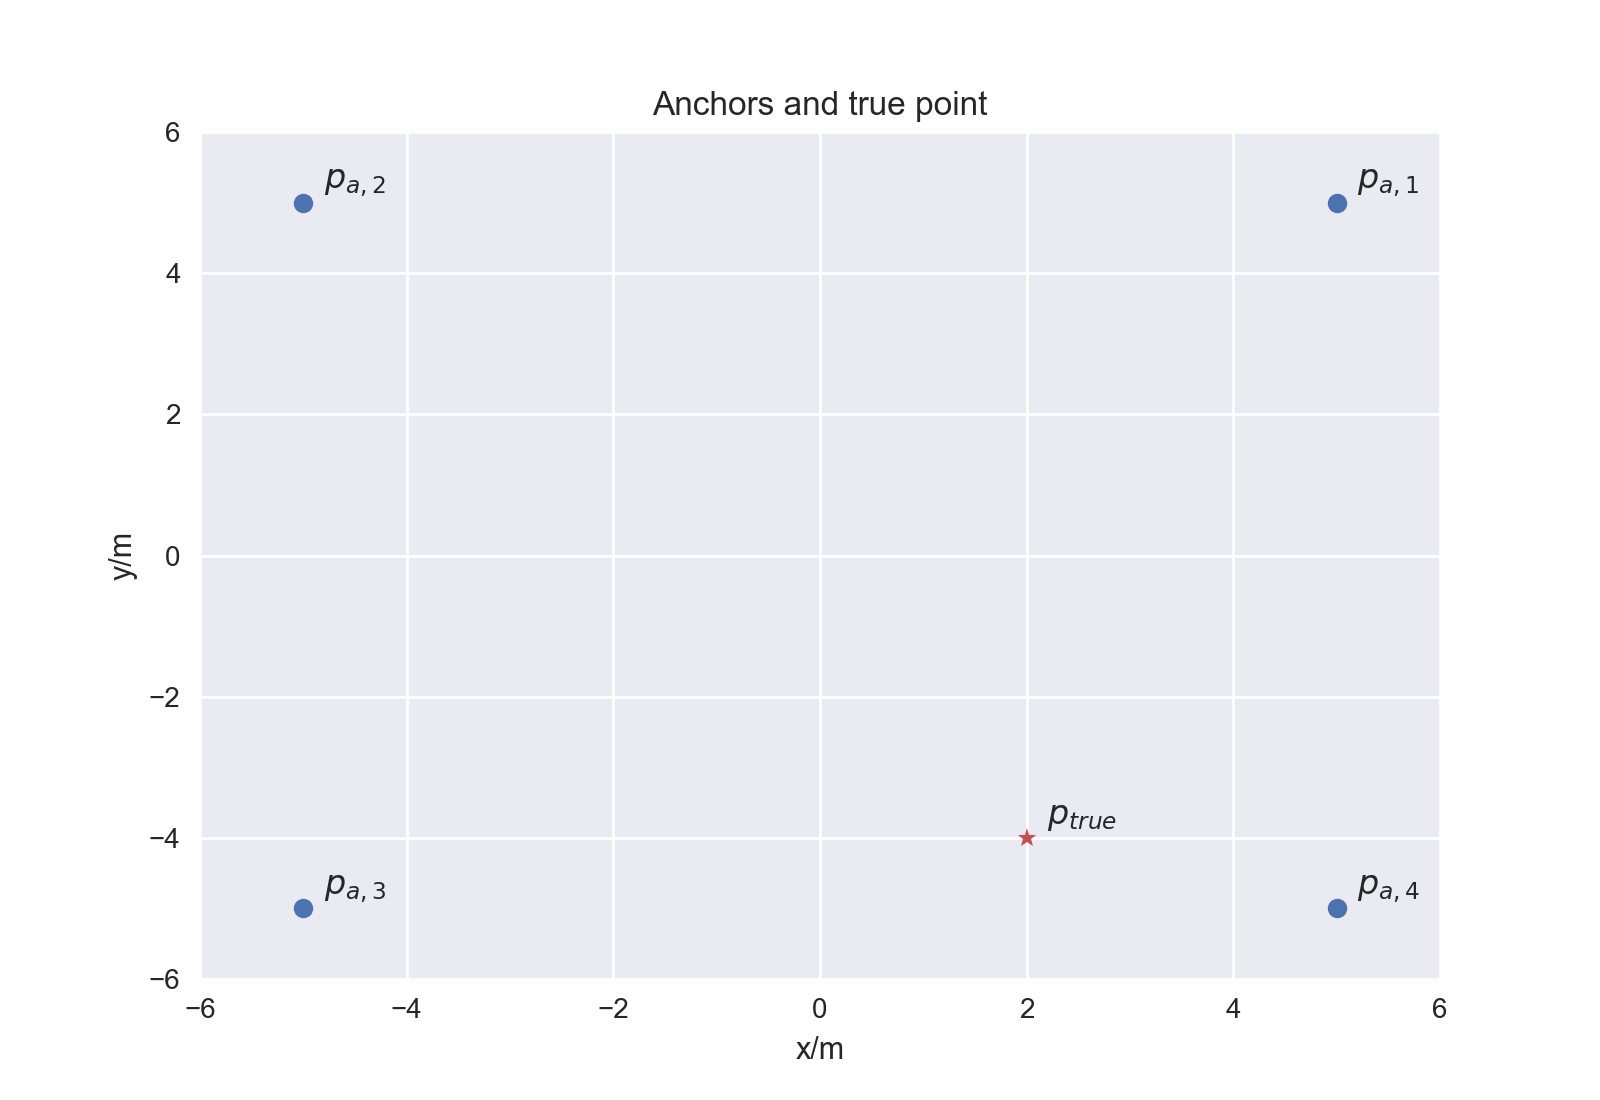
\includegraphics[width=14cm]{anchors_and_true_point.png}
	\caption{Anchors and True point.}
	\label{fig1:points}
\end{figure}

Note that we increased the anchor indices by $1$ for better understanding.

\subsection{For scenario 2, find out which is the anchor with exponentially distributed measurements.}
To find out which is the anchor with exponentially distributed measurements, we took all measurements for each anchor separately and plotted them in a distribution histogram.

\begin{figure}[H]
	\centering
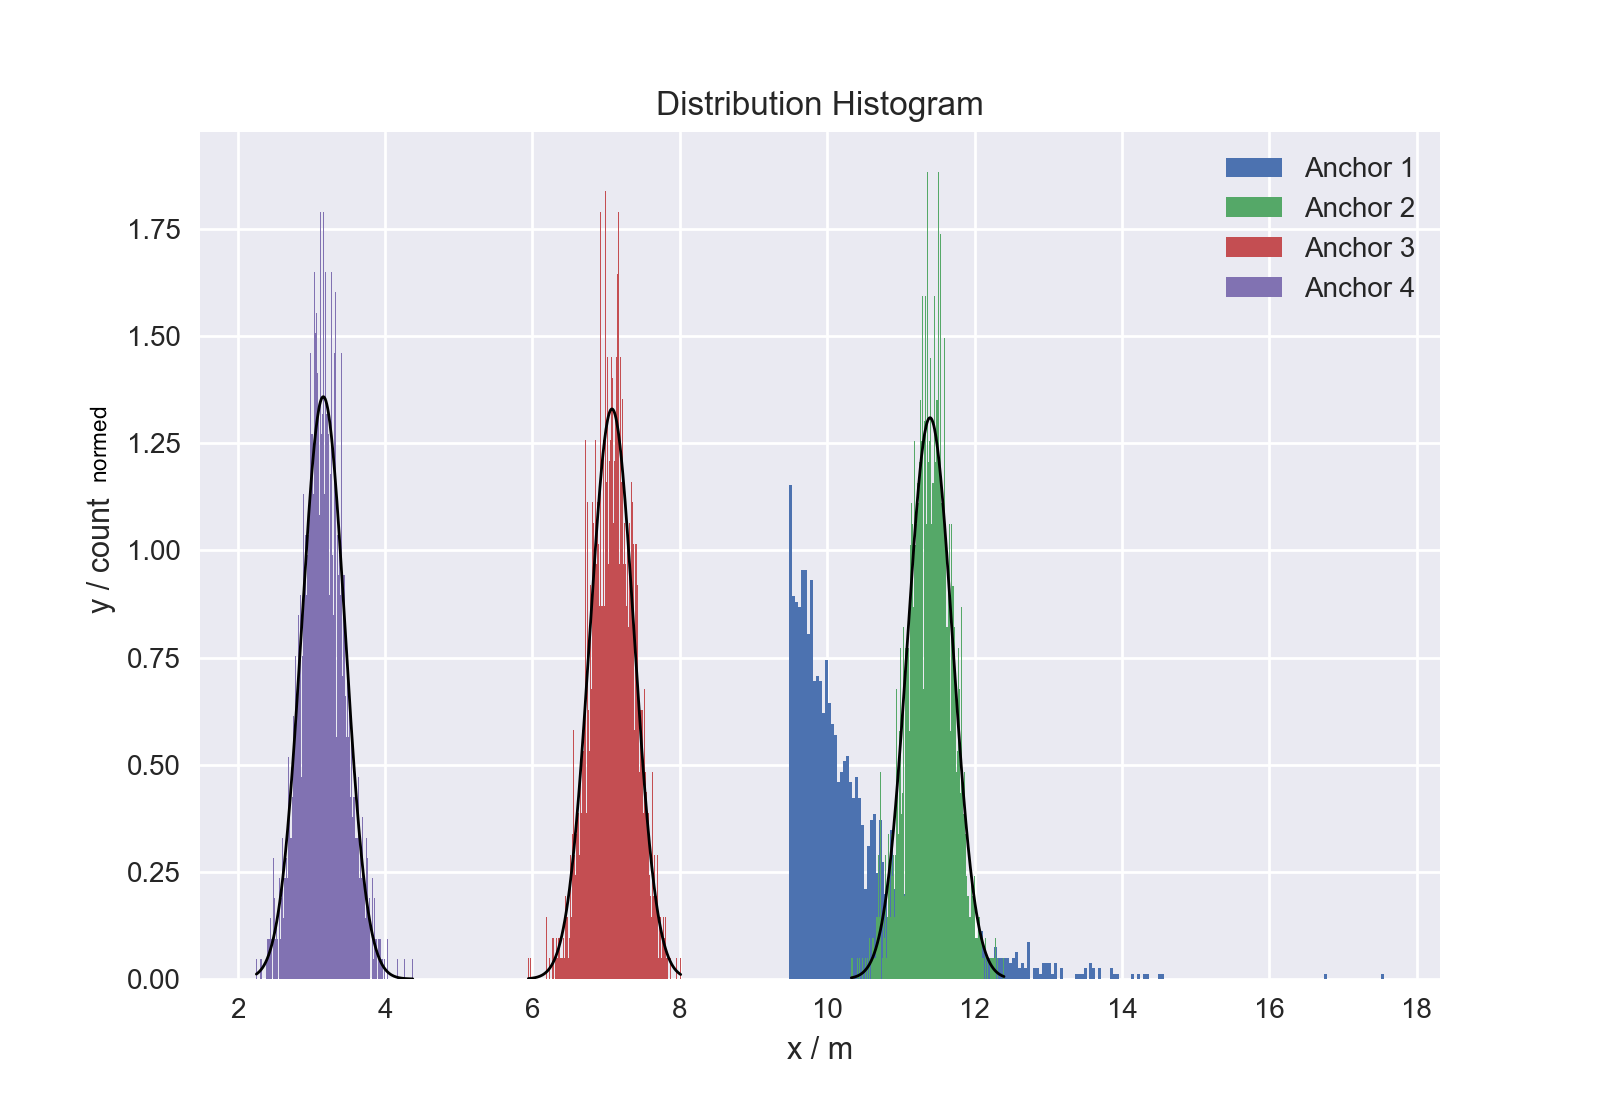
\includegraphics[width=14cm]{histogram.png}
	\caption{Distribution Histogram of measurements per anchor for scenario 2.}
	\label{fig1:histogram}
\end{figure}

Using this histogram, we could conclude that Anchor 1 is the anchor with exponentially distributed measurements as seen in Figure ~\ref{fig1:histogram} 

\subsection{Analytically derive the maximum likelihood solution for the exponential distribution.}

The maximum likelihood estimator is given as 

\begin{align*}
\hspace*{2cm}
\mathbf{\hat{p}}_{ML} = argmax \prod\limits_{i=1}^N p(r_i|\mathbf{p})
\end{align*}

and the exponential distribution is given as

\begin{align*}
\hspace*{2cm}
p(r_i|\mathbf{p}) = \lambda_i \exp{-\lambda_i(r_i-d_i(\mathbf{p}))} \quad for \quad r_i \geq d_i(\mathbf{p}), \quad else \quad 0.
\end{align*}

The analytical derivation of the maximum likelihood solution for the exponential distribution is performed as followed:

\begin{align*}
\hspace*{2cm}
\mathbf{\hat{p}}_{ML} &= argmax \prod\limits_{i=1}^N p(r_i|\mathbf{p})\\
&= argmax \quad \lambda_i^N \exp{-\lambda_i \sum\limits_{i=1}^N (r_i-d_i(\mathbf{p}))}
\end{align*}

We now perform an $ln$ operation, as $ln$ is monoton rising, and therefor not changing anything for the argmax function.

\begin{align*}
\hspace*{2cm}
ln(\mathbf{\hat{p}}_{ML}) &= argmax \quad ln(\lambda_i^N) + -\lambda_i \sum\limits_{i=1}^N (r_i-d_i(\mathbf{p}))\\
&= argmax \quad N ln(\lambda_i) - \lambda_i \sum\limits_{i=1}^N (r_i-d_i(\mathbf{p}))
\end{align*}

To find the optimal value for $\lambda_i$, we derive $ln(\mathbf{\hat{p}}_{ML})$ for $\lambda_i$. This derivation should equal $0$, so that we get the maximum.

\begin{align*}
\hspace*{2cm}
\dfrac{\partial ln(\mathbf{\hat{p}}_{ML})}{\partial\lambda_i} = \dfrac{N}{\lambda_i} - \sum\limits_{i=1}^N (r_i-d_i(\mathbf{p})) \stackrel{!}{=} 0
\end{align*}

From here we conclude our final solution for $\lambda_i$:

\begin{align*}
\hspace*{2cm}
\lambda_i = \dfrac{N}{\sum\limits_{i=1}^N (r_i-d_i(\mathbf{p}))}
\end{align*}



\subsection{Estimate the parameters of the measurement models for all anchors in all 3 scenarios using the maximum likelihood method.}

We estimated the parameters for all 3 scenarios and came to the following results:

\begin{figure}[H]
	\centering
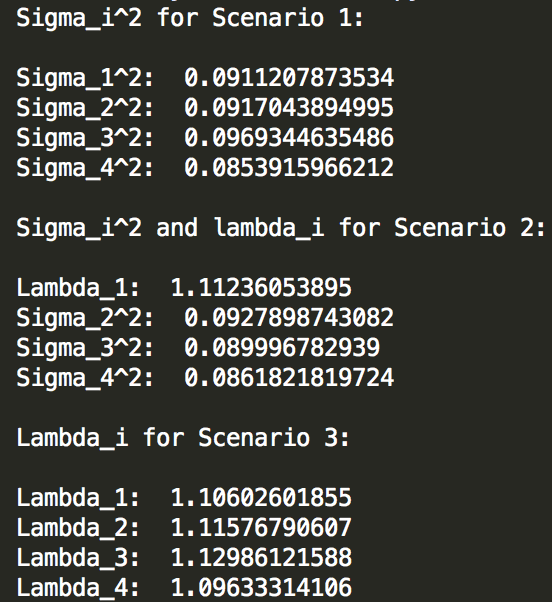
\includegraphics[width=10cm]{estimated_params.png}
	\caption{Estimated parameters for all 3 scenarios.}
	\label{fig1:params}
\end{figure}

\section{Least-Squares Estimation of the Position}
\subsection{Show analytically that for scenario 1 (joint likelihood for the distances is Gaussian), the least-squares estimator of the position is equivalent to the maximum likelihood estimator}

The maximum likelihood estimator is given as:

\begin{align*}
\hspace*{2cm}
\mathbf{\hat{p}}_{ML} = argmax \prod\limits_{i=1}^N p(r_i|\mathbf{p})
\end{align*}

We further perform an $ln$ operation, as $ln$ is monoton rising, and therefor not changing anything for the argmax function.

\begin{align*}
\hspace*{2cm}
\mathbf{\hat{p}}_{ML} &= argmax \prod\limits_{i=1}^N p(r_i|\mathbf{p})\\ 
&= argmax \sum\limits_{i=1}^N ln(p(r_i|\mathbf{p}))\\
&= argmax \sum\limits_{i=1}^N ln\Bigg[\dfrac{1}{\sqrt{2\pi\sigma_i^2}} \exp{-\dfrac{(r_i-d_i(\mathbf{p}))^2}{2\sigma_i^2}}\Bigg]\\
\end{align*}

To continue, we use the following relation: 
$argmax f(x) = argmin - f(x)$

\begin{align*}
\hspace*{2cm}
\mathbf{\hat{p}}_{ML} &= argmax \sum\limits_{i=1}^N ln\Bigg[\dfrac{1}{\sqrt{2\pi\sigma_i^2}} \exp{-\dfrac{(r_i-d_i(\mathbf{p}))^2}{2\sigma_i^2}}\Bigg]\\
&= argmin - \sum\limits_{i=1}^N \Bigg[ln\bigg(\dfrac{1}{\sqrt{2\pi\sigma_i^2}}\bigg) + ln\bigg(\exp{-\dfrac{(r_i-d_i(\mathbf{p}))^2}{2\sigma_i^2}}\bigg)\Bigg]\\
&= argmin - \sum\limits_{i=1}^N \Bigg[ln\bigg(\dfrac{1}{\sqrt{2\pi\sigma_i^2}}\bigg) - \dfrac{(r_i-d_i(\mathbf{p}))^2}{2\sigma_i^2}\Bigg]\\
\end{align*}

Because a constant does not change anything for the argmin function, because it is changing every argument in a linear way, we can neglect the constant:

\begin{align*}
\hspace*{2cm}
\mathbf{\hat{p}}_{ML} &= argmin - \sum\limits_{i=1}^N \Bigg[ln\bigg(\dfrac{1}{\sqrt{2\pi\sigma_i^2}}\bigg) - \dfrac{(r_i-d_i(\mathbf{p}))^2}{2\sigma_i^2}\Bigg]\\
&\approx argmin - \sum\limits_{i=1}^N \Bigg[- \dfrac{(r_i-d_i(\mathbf{p}))^2}{2\sigma_i^2}\Bigg]\\ 
&\approx argmin  \sum\limits_{i=1}^N \Bigg[\dfrac{(r_i-d_i(\mathbf{p}))^2}{2\sigma_i^2}\Bigg]\\
\end{align*}

Now, the constant can be again neglected, as it is not influencing the argmin function, and we can make the final step:

\begin{align*}
\hspace*{2cm}
\mathbf{\hat{p}}_{ML} \approx argmin \sum\limits_{i=1}^N (r_i-d_i(\mathbf{p}))^2 \approx \mathbf{\hat{p}}_{LS}\\
\end{align*}

As one can see, the least-squares estimator of the position is equivalent to the maximum likelihood estimator (for the gaussian model).

\subsection{Implement the Gauss-Newton algorithm to find the least-squares estimate for the position and write a function LeastSquaresGN. You may choose suitable values for the tolerance and the maximum number of iterations on your own. The output is the estimated position.}

The functionality of the written function will be verified and used in Point 2.3.
We set max\_iter to $20$ and tol to $10^{-3}$.
For the Jacobi Matrix, the following derivates were used:

\begin{align*}
\hspace*{2cm}
\dfrac{\partial(r_i-d_i(\mathbf{p}))}{\partial x} = \dfrac{x_i - x}{\sqrt{(y_i - y)^2 + (x_i - x)^2}}\\
\end{align*}
\begin{align*}
\hspace*{2cm}
\dfrac{\partial(r_i-d_i(\mathbf{p}))}{\partial y} = \dfrac{y_i - y}{\sqrt{(y_i - y)^2 + (x_i - x)^2}}\\
\end{align*}



\subsection{For all three scenarios, evaluate your estimation algorithm using the provided data. For each of the N = 2000 independent measurements, choose the starting position p0 randomly according to a uniform distribution within the square spanned by the anchor points.}

\subsubsection{The mean and variance of the position estimation error.}

\begin{figure}[H]
	\centering
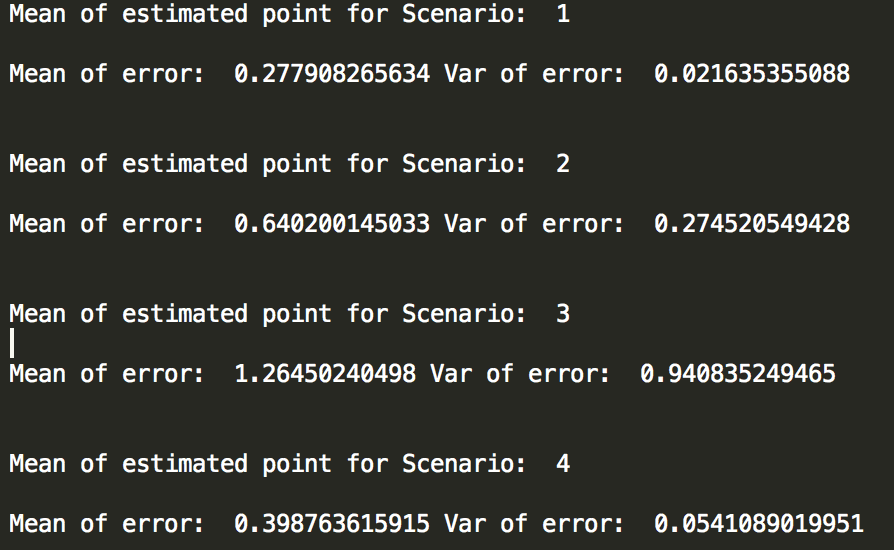
\includegraphics[width=10cm]{mean_var_calc.png}
	\caption{Mean and variance of the position estimation error for 4 scenarios, where the forth scenario only uses 3 gaussian anchors (exponential anchor was deleted).}
	\label{fig1:meanvariance}
\end{figure}

\subsubsection{Scatter plots of the estimated positions. Fit a two-dimensional Gaussian distribution to the point cloud of estimated positions and draw its contour lines. Do the estimated positions look Gaussian? What can you say about the probability of large estimation errors?}

\begin{figure}[H]
	\centering
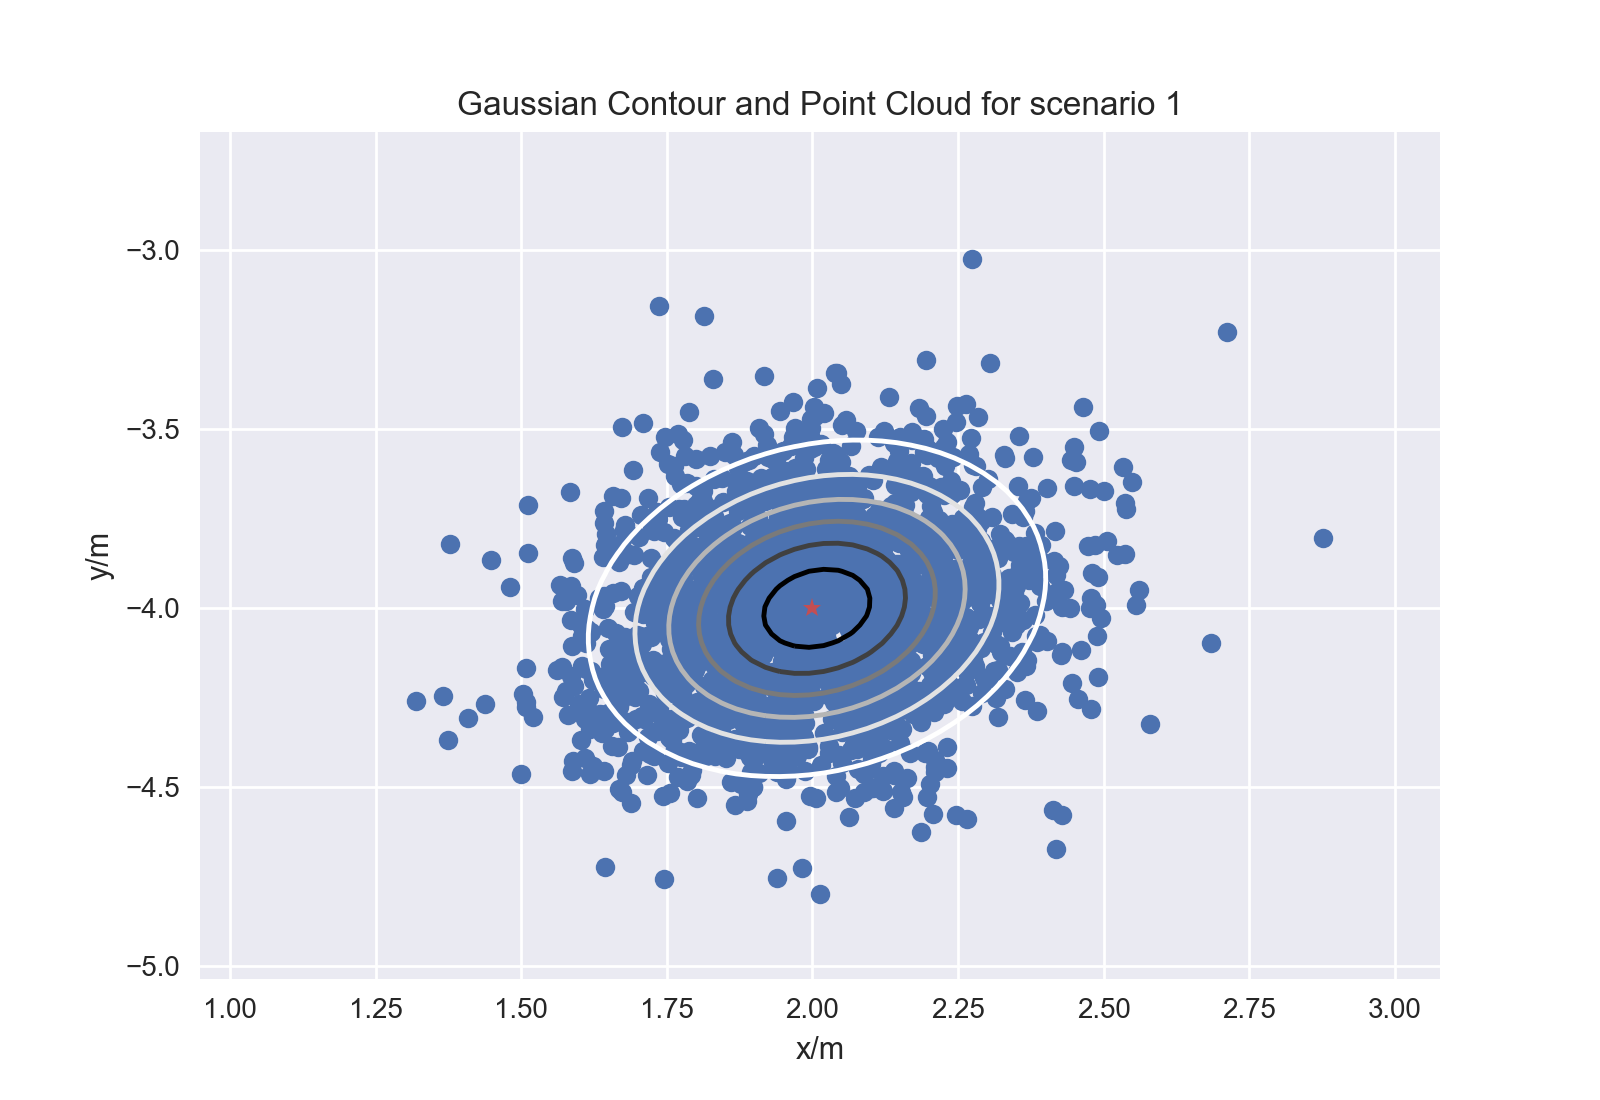
\includegraphics[width=14cm]{gauss1.png}
	\caption{Gaussian contour and point cloud for scenario 1.}
	\label{fig1:gpc1}
\end{figure}

\begin{figure}[H]
	\centering
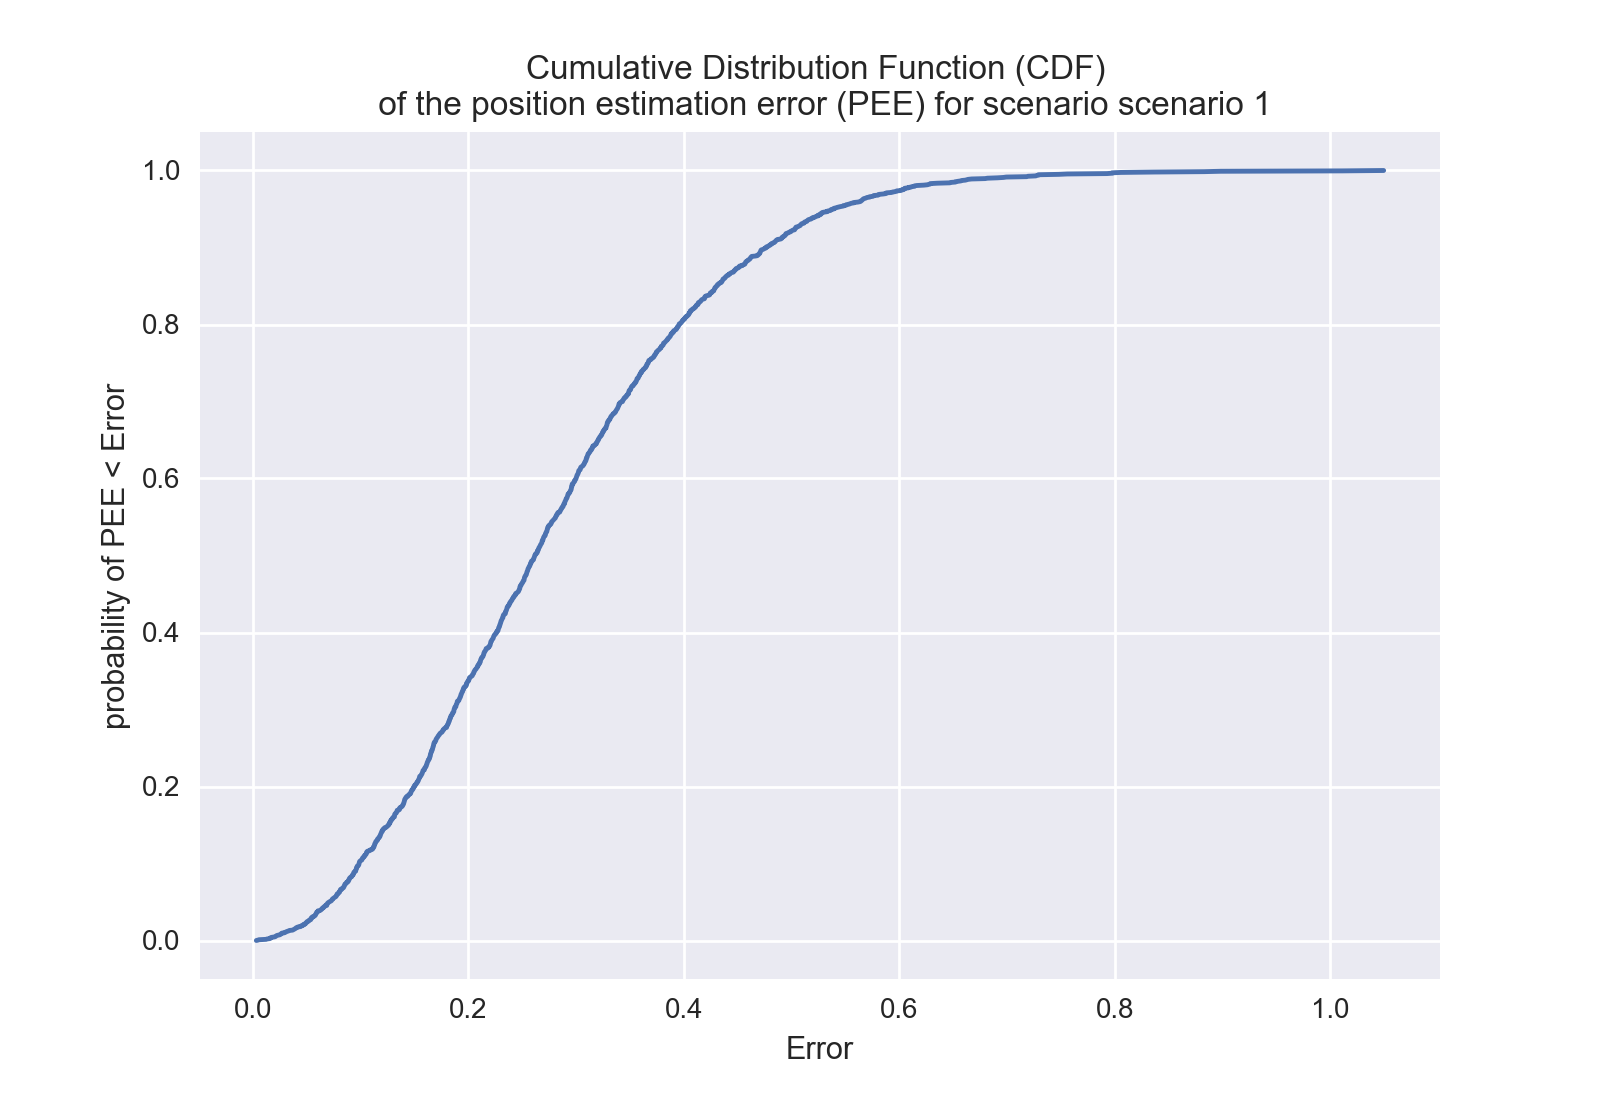
\includegraphics[width=14cm]{cdf1.png}
	\caption{Cumulative Distribution Function of the position estimation error for scenario 1.}
	\label{fig1:cdf1}
\end{figure}

\begin{figure}[H]
	\centering
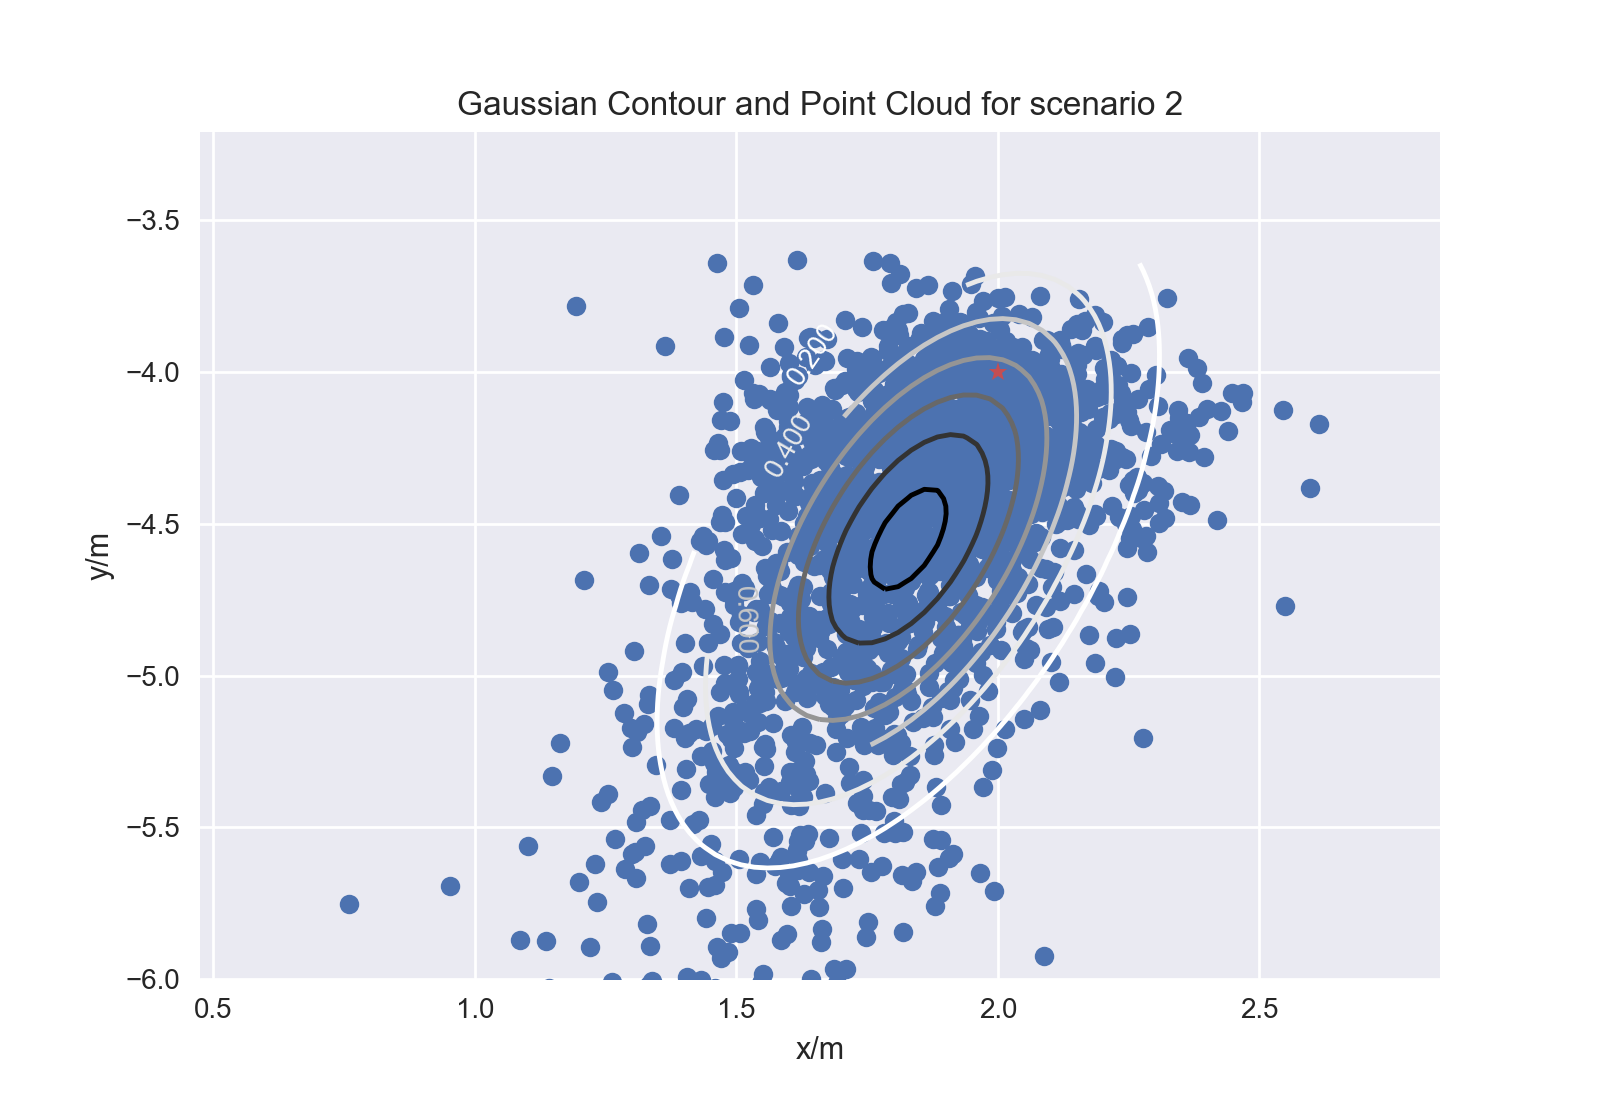
\includegraphics[width=14cm]{gauss2.png}
	\caption{Gaussian contour and point cloud for scenario 2.}
	\label{fig1:gpc2}
\end{figure}

\begin{figure}[H]
	\centering
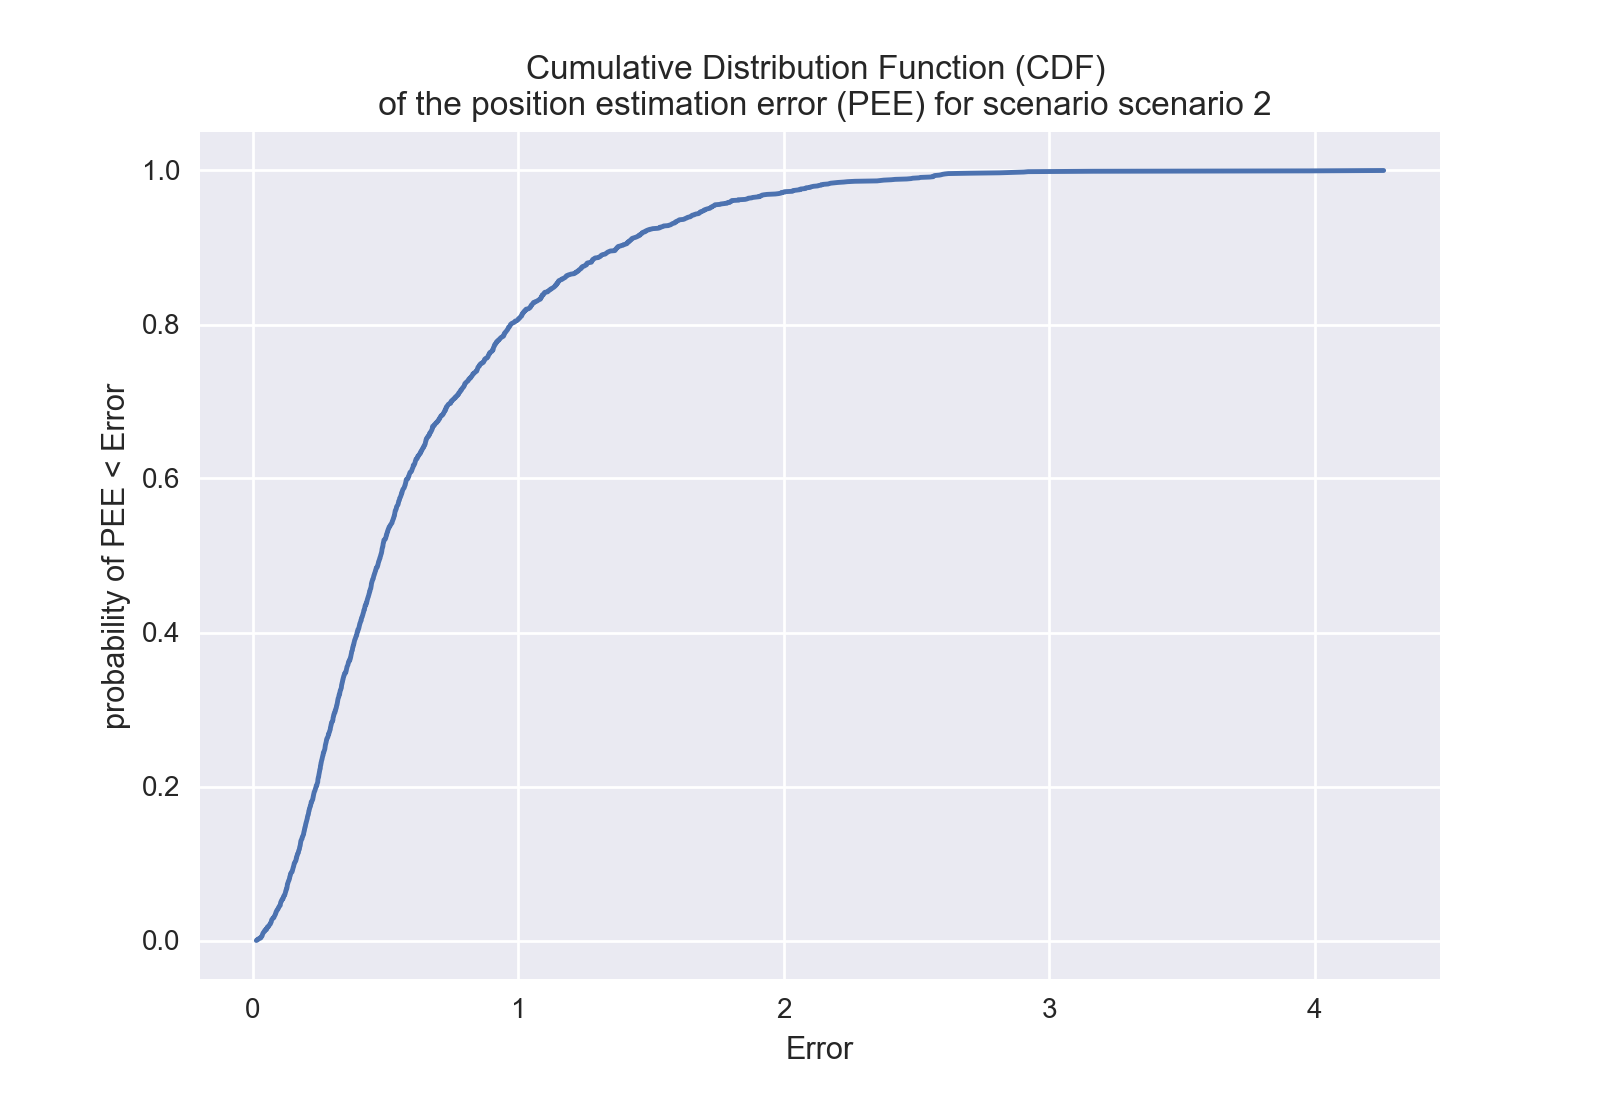
\includegraphics[width=14cm]{cdf2.png}
	\caption{Cumulative Distribution Function of the position estimation error for scenario 2.}
	\label{fig1:cdf2}
\end{figure}

\begin{figure}[H]
	\centering
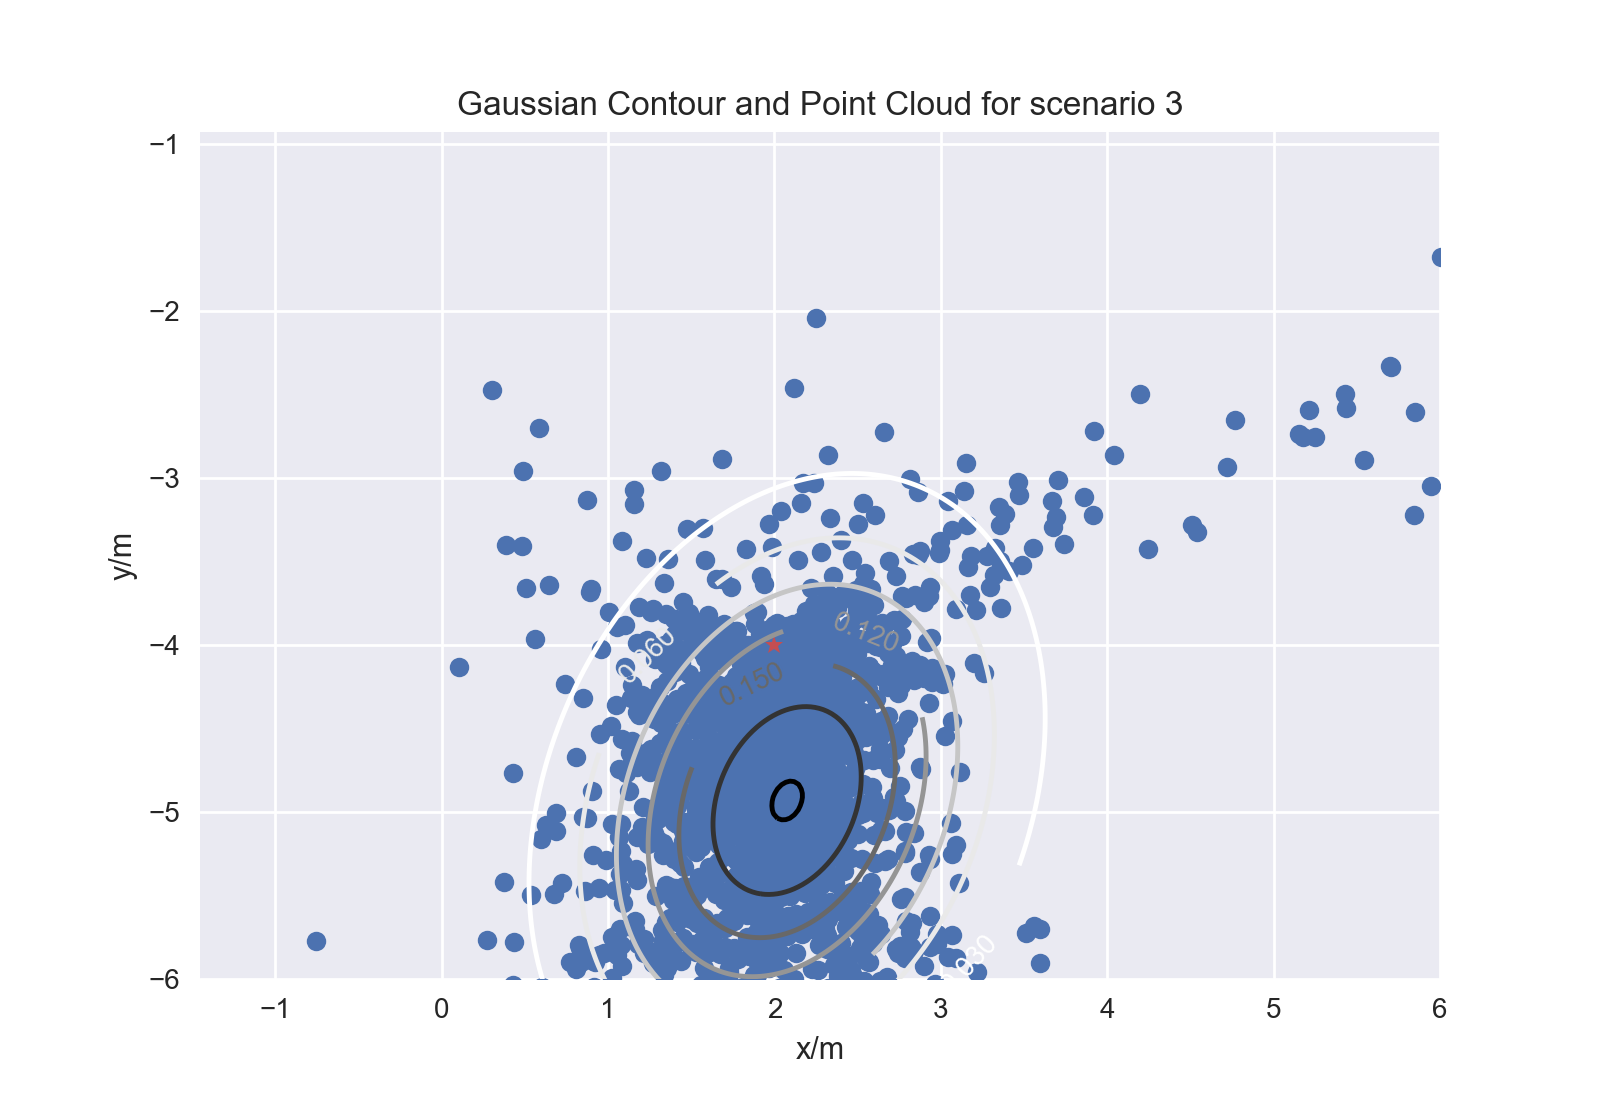
\includegraphics[width=14cm]{gauss3.png}
	\caption{Gaussian contour and point cloud for scenario 3.}
	\label{fig1:gpc3}
\end{figure}

\begin{figure}[H]
	\centering
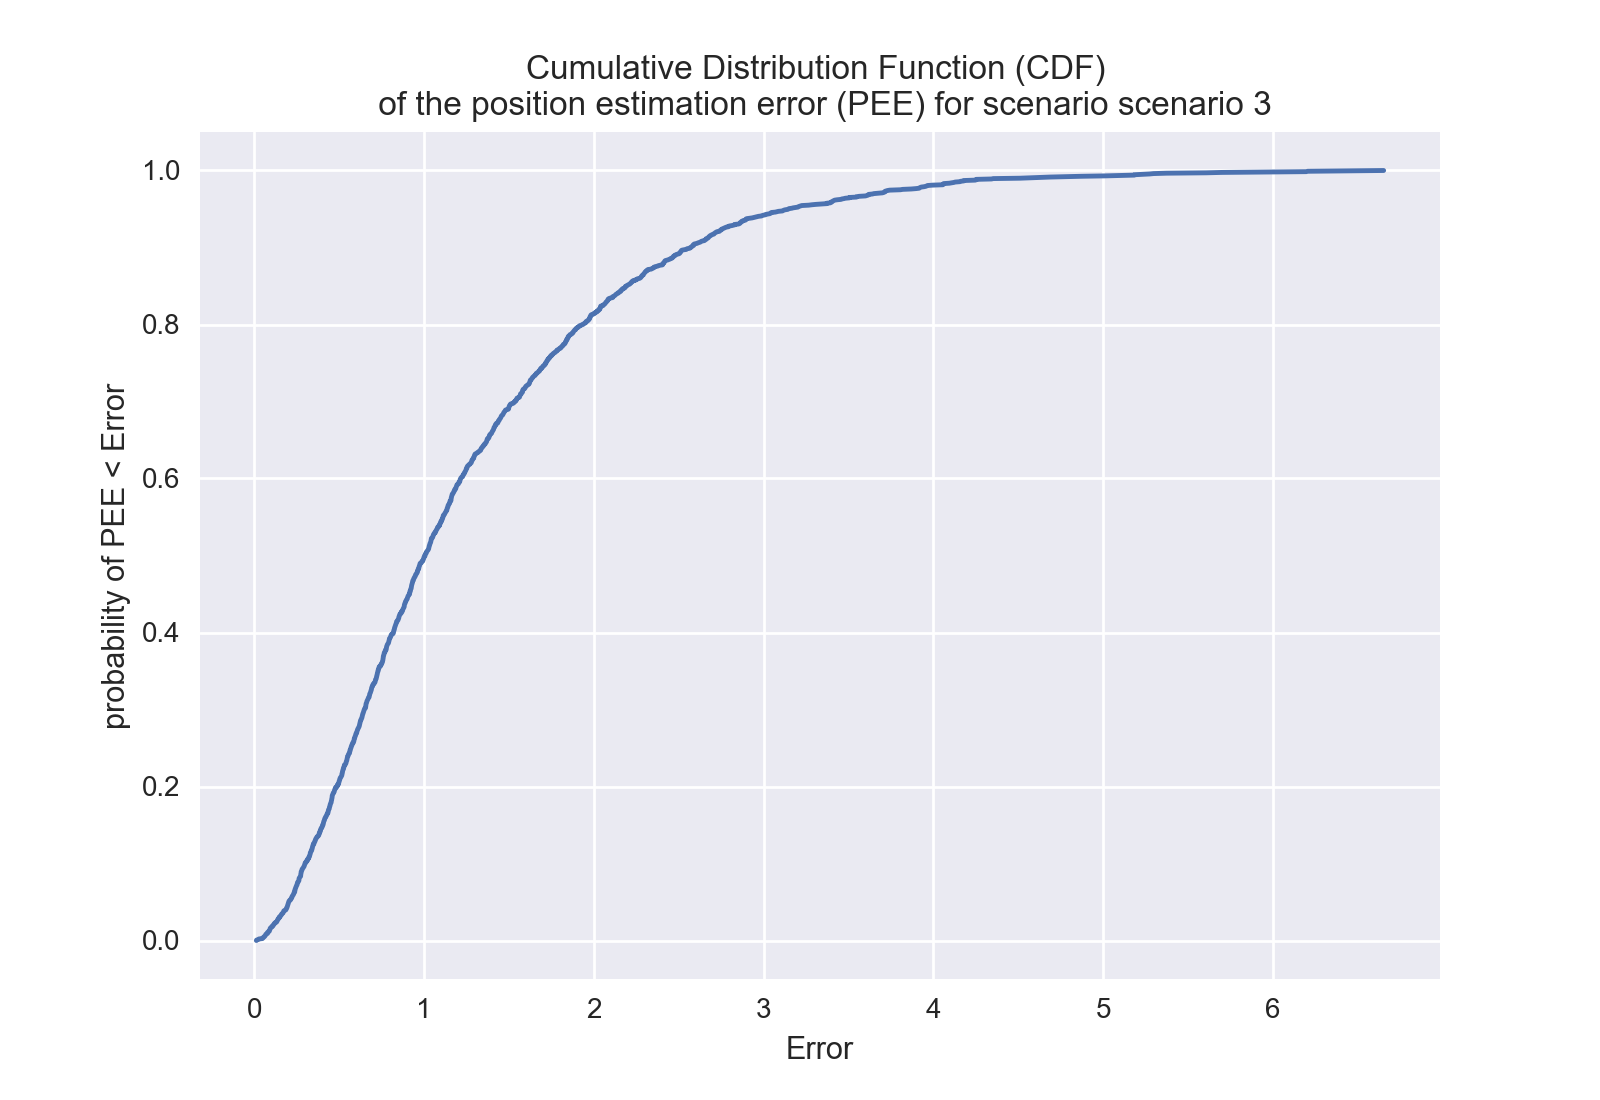
\includegraphics[width=14cm]{cdf3.png}
	\caption{Cumulative Distribution Function of the position estimation error for scenario 3.}
	\label{fig1:cdf3}
\end{figure}

\begin{figure}[H]
	\centering
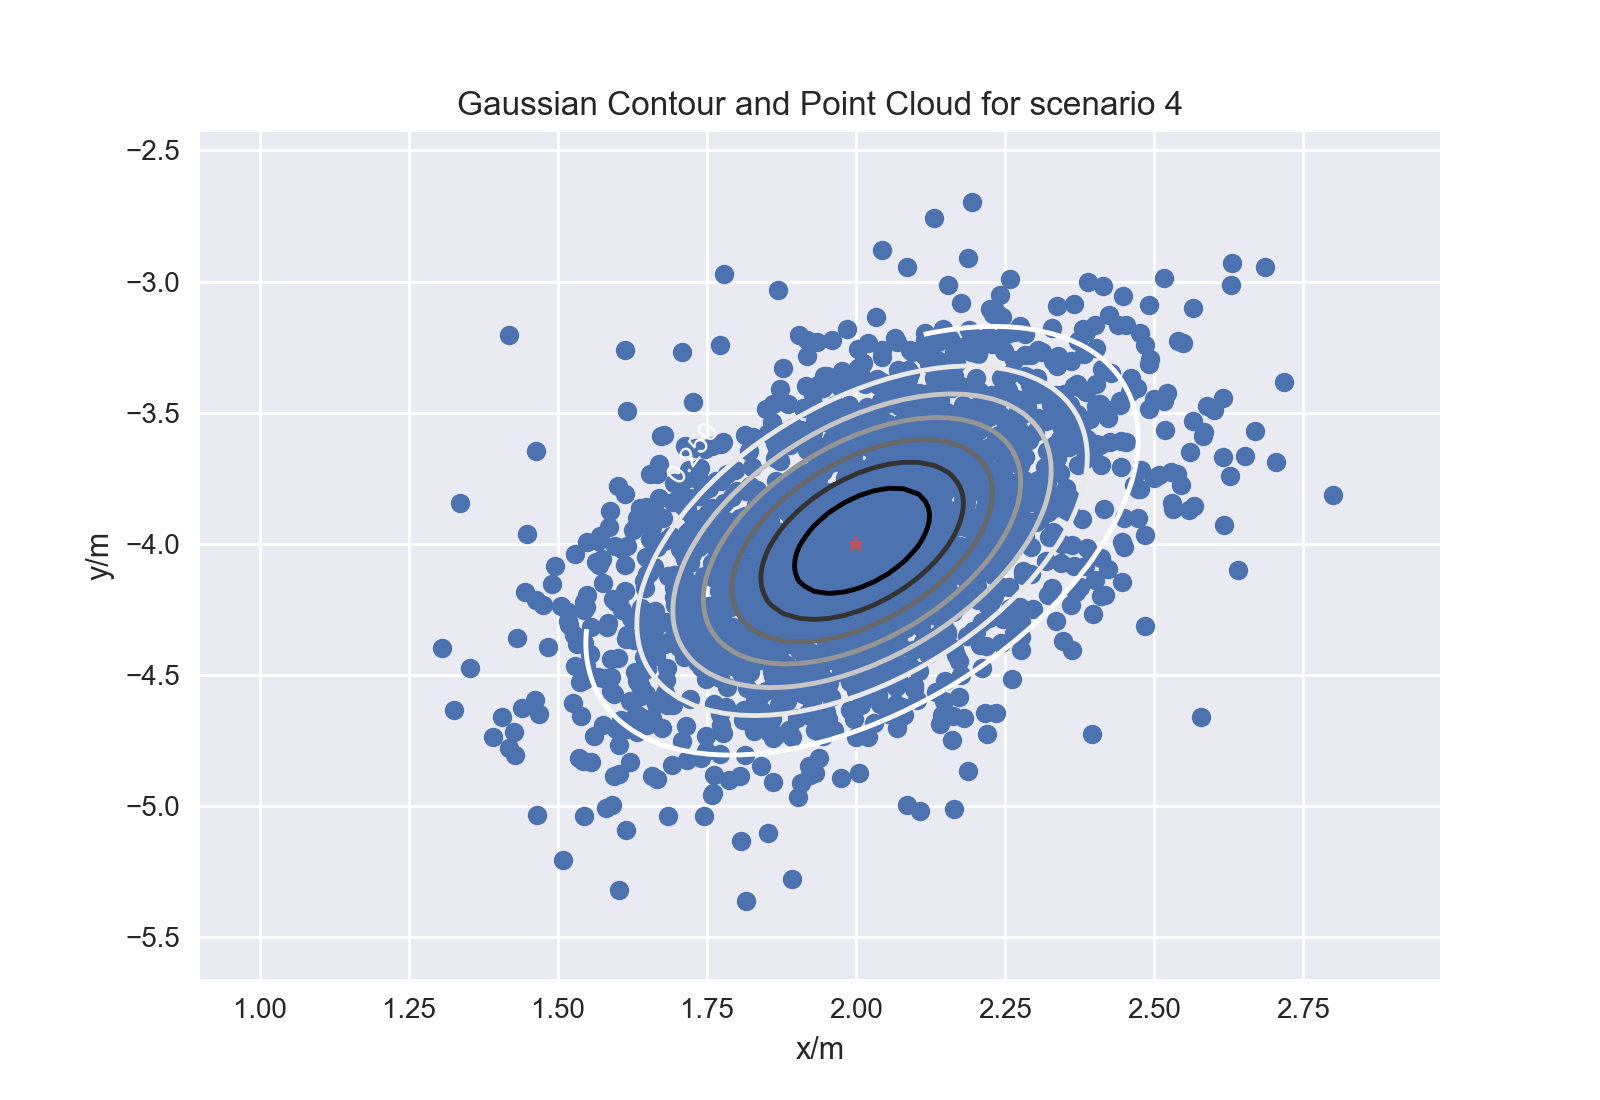
\includegraphics[width=14cm]{gauss4.png}
	\caption{Gaussian contour and point cloud for scenario 4.}
	\label{fig1:gpc4}
\end{figure}

\begin{figure}[H]
	\centering
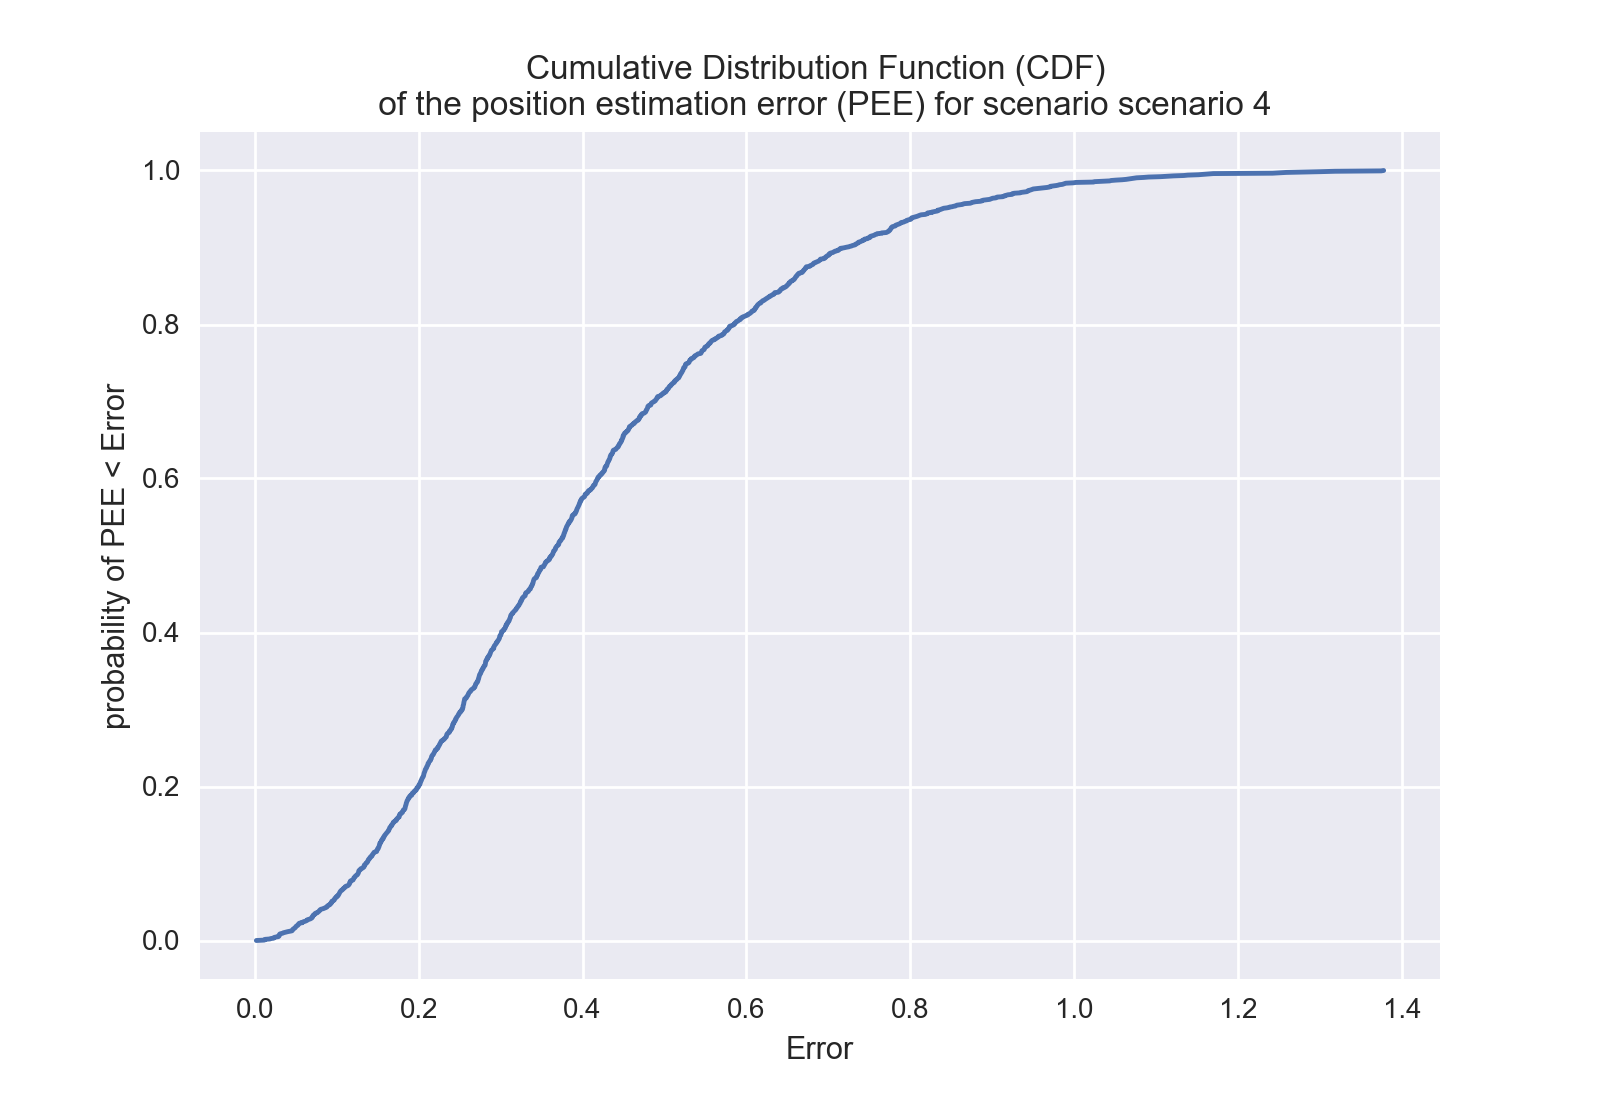
\includegraphics[width=14cm]{cdf4.png}
	\caption{Cumulative Distribution Function of the position estimation error for scenario 4.}
	\label{fig1:cdf4}
\end{figure}

As one can see in the plots, the estimated points for scenario 1 and 4 look gaussian. This is because there are only gaussian anchors. The estimated points for scenario 2 and 3 do not really look gaussian, as there are a lot of points far away from the gaussian contour.\\

By looking at the CDF plots, we can see, that for scenario 1 and 4 (gaussian anchors) the probability for the error being smaller than 0.8 and 1.4 respectively is nearly 100\%.
For scenario 2 and 3 , where we have at least one exponential anchor, we can say with a high probability that our position estimation error is much greater than in the gaussian examples.\newpage

The following plot shows then mean of the estimated point cloud for each scenario.

\begin{figure}[H]
	\centering
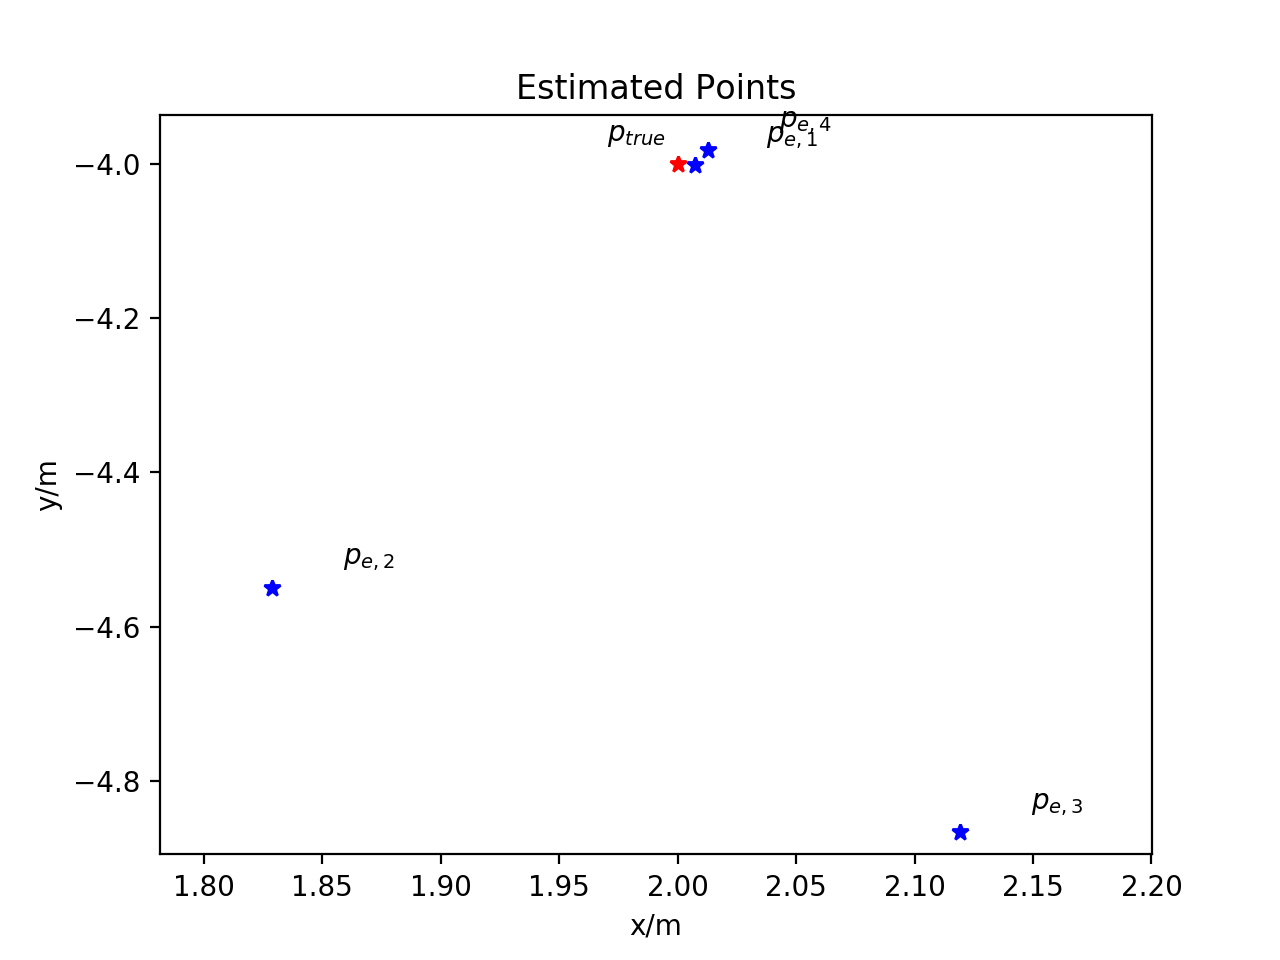
\includegraphics[width=14cm]{estimated_points.png}
	\caption{Mean estimated points for each scenario (magnified).}
	\label{fig1:meanpoints}
\end{figure}

\subsection{Compare the performance of scenario 2 with scenario 4. What can you observe?}
By looking at our plots, we conclude that we get a lower position estimation error for scenario 4 compared to scenario 2. This effect can be seen again in Figure ~\ref{fig1:meanvariance}, where scenario 4 performs better because it has a lower mean and variance of estimation errors.
\newpage

\section{Numerical Maximum-Likelihood Estimation of the Position}

\subsection{For the first measurement (i.e. the first NA distance estimates), compute the joint likelihood function over a two dimensional grid with a resolution of 5 cm. Confine the evaluation to the square region that is enclosed by the anchors. Why might it be hard to find the maximum of this function with a gradient ascent algorithm using an arbitrary starting point within the evaluation region? Is the maximum at the true position?}

First, we computed the joint likelihood function

\begin{align*}
\hspace*{2cm}
\mathbf{\hat{p}}_{ML} = argmax \prod\limits_{i=1}^N \lambda_i \exp{-\lambda_i(r_i-d_i(\mathbf{p}))}
\end{align*}

and then we evaluated it for the first measurement of our given data.

\begin{figure}[H]
	\centering
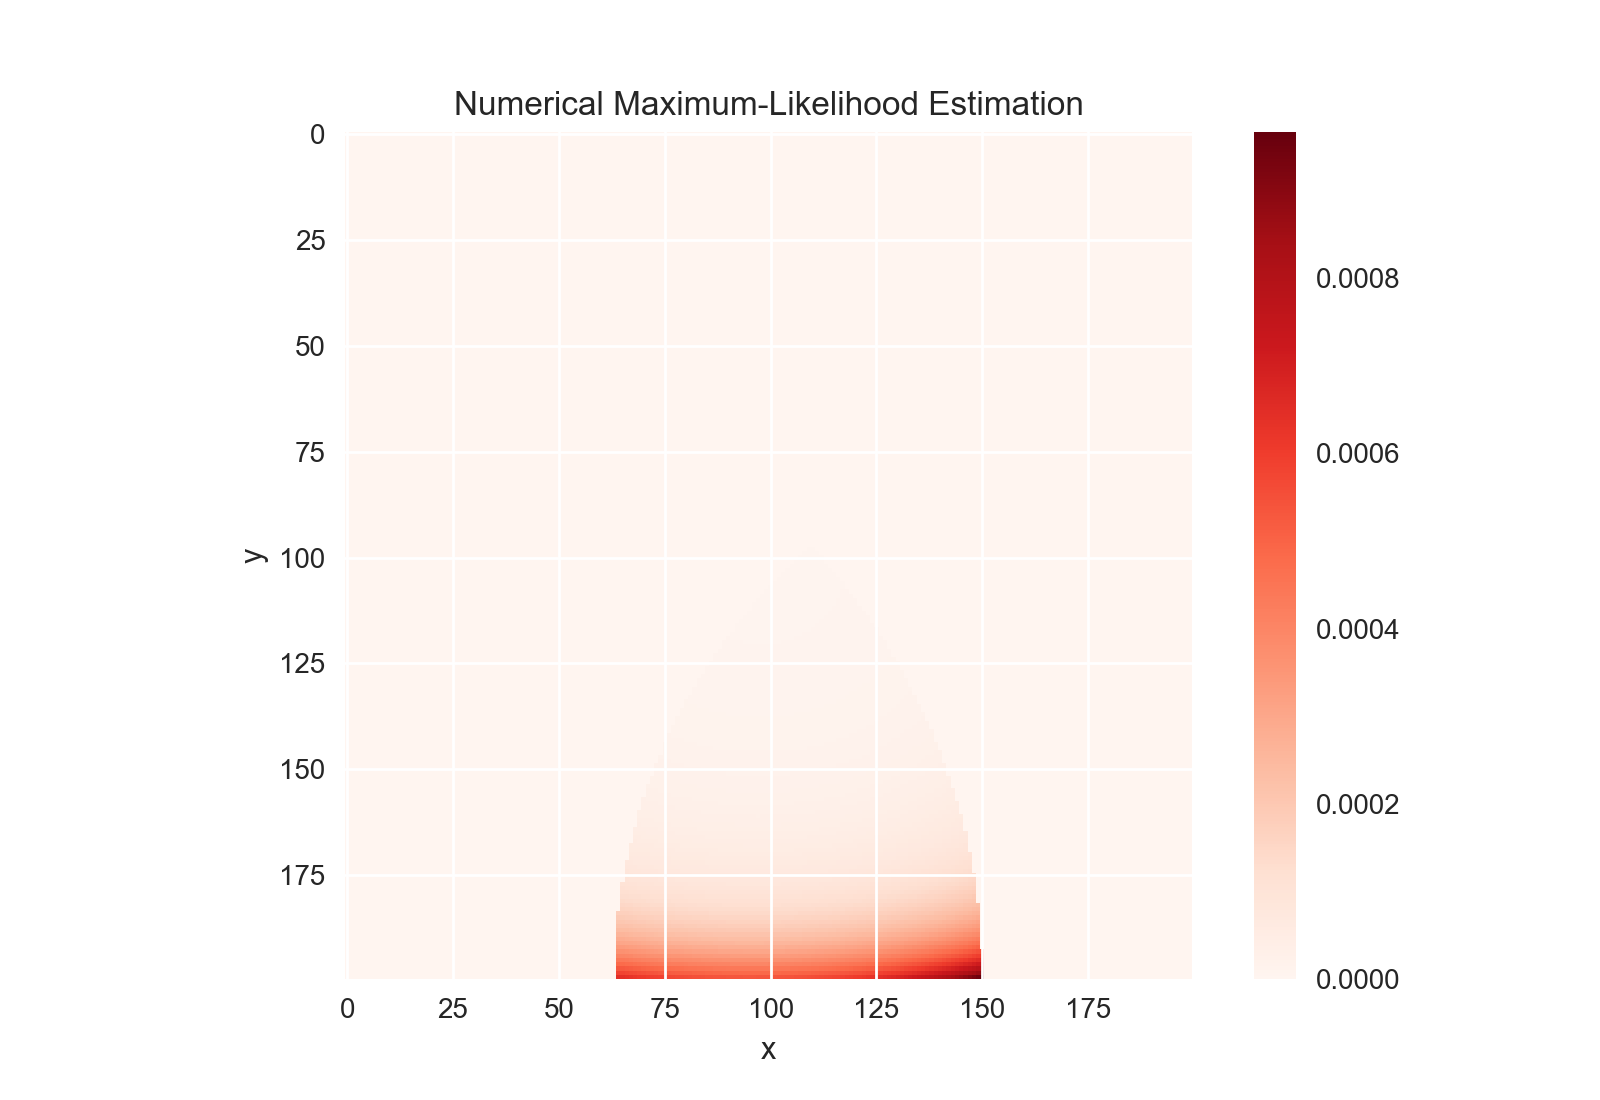
\includegraphics[width=18cm]{numerical_maximum.png}
	\caption{Numerical maximum likelihood estimation.}
	\label{fig1:nummax}
\end{figure}

In this Figure we can see that the numerical maximum likelihood estimator is a non-convex function and therefore a gradient ascent algorithm would get stuck in local maxima quiet easily. 
The maximum is not at the true position (2,-4), instead it is at (2.5, -4.95).

% **************************************************************************************************
%\appendix
% \bibliographystyle{./base/IEEEtran}
% \bibliography{_bibliography}


% **************************************************************************************************
% **************************************************************************************************

% place all floats and create label on last page
\FloatBarrier\label{end-of-document}
\end{document}

